\chapter{Aprendizagem}
\label{cap4}
\par Neste capitulo serão apresentadas alguns exemplos realizados antes de iniciar o desenvolvimento do projecto, com o objectivo de adquirir alguns conhecimentos nas tecnologias a utilizar, visto que até à data de inicio do projecto a experiência era reduzida nas mesmas.

\section{AngularJS e D3.js}
\par Apesar de já ter uma reduzida experiência com a framework de javascript AngualrJS, não detinha qualquer experiência com a biblioteca de gráficos javascript D3.js. Por esse motivo foi necessário realizar na primeira fase, um pequeno projecto que me permitisse obter alguns conhecimentos acerca desta duas tecnologias, para mais tarde aplicar esses mesmos conhecimentos no desenvolvimento do projeto. \newline
A Listagem \ref{example:angular} apresenta o código desenvolvido para o exemplo. Para a apresentação do gráfico na página decidi criar uma diretiva, recurso da \textit{framework} \textit{AngularJS}, que muito sucintamente se comporta como se fosse um \textit{template}, que é alimentado por parâmetros, como podemos visualizar na Listagem \ref{example-angulaCtrl}.
\begin{lstlisting}[language=html,caption={Código fonte da primeira página em AngularJS},{label=example:angular}]
<!DOCTYPE html>
<html>
<head>
    <meta charset=utf-8 />
    <script src="/js/angular.min.js"></script>
    <script src="/js/d3.js"></script>
    <script src="/js/d3plus.js"></script>
    <link href="/css/bootstrap.min.css" rel="stylesheet" type="text/css" />
    <script src="/js/main_controller.js"></script>
    <title>Angular JS Demo</title>
</head>
<body ng-app="start" ng-controller="mainController" class="text-center">
    <h2 ng-bind="title"></h2>
    <div class="col-lg-6 col-md-6">
        <pie-chart id="viz" data="data" width="400" height="400"></pie-chart>
    </div>
    <div class="col-lg-6 col-md-6">
        <div class="input-group" ng-repeat="data in data">
            <span class="input-group-addon" id="sizing-addon2" ng-bind="data.name"></span>
            <input type="number" class="form-control" placeholder="{{data.name}}" aria-describedby="sizing-addon2" ng-model="data.value">{{data.value}}
        </div>
    </div>
</body>
</html>
\end{lstlisting}

\begin{lstlisting}[language=html,caption={Directiva e Controller AngularJS},{label=example:angulaCtrl}]
(function () {
    var app = angular.module('start', []);
    home.directive('pieChart', function ($compile) {
        return {
            restrict: 'E',
            scope: {
                data: '=?',
                width: '=?',
                height: '=?',
            },
            compile: function (element, attributes) {
                if (!attributes.height) {
                    attributes.height = 200;
                }
                post: function postLink($scope, element /*, attributes*/ ) {
                    $scope.$watch('data', function (newVals, oldVals) {
                        updatePie($scope, element);
                    }, true);
                }
                return postLink;
            }
        }
    });

    app.controller('mainController', ['$scope', function ($scope) {
        $scope.title = "Primeiro exemplo D3.js/AngularJS";
        $scope.data = [
            {"value": 100, "name": "alpha"},
            {"value": 70, "name": "beta"},
            {"value": 40, "name": "gamma"},
            {"value": 15, "name": "delta"},
            {"value": 5, "name": "epsilon"},
            {"value": 1, "name": "zeta"}
        ];
    }]);

    function updatePie($scope, element) {
        d3plus.viz()
            .container("#" + element[0].id)
            .data($scope.data)
            .type("pie")
            .id("name")
            .size("value")
            .width($scope.width)
            .height($scope.height)
            .draw()
    }
})();
\end{lstlisting}


\section{Primeira aplicação em \textit{QlikView}}
\par No que respeita ao \textit{QlikView} foi uma experiência completamente nova, pois até à data de inicio do projecto não tinha qualquer experiência, desconhecendo mesmo esta ferramenta de \textit{reporting}. Como tal foi necessário despender algum tempo para investigação, e aprendizagem autónoma, de forma a conseguir desenvolver uma pequena aplicação de teste, que me serviu de ponto de partida. O contributo do cliente foi muito importante ao disponibilizar uma aplicação já existente, pois através da sua exploração consegui adquirir os conhecimentos básicos para avançar nesta tecnologia.\newline
\par Para um primeiro exemplo, utilizei como fonte de dados um documento em formato \textit{.xlsx}, com uma listagem de equipamentos, em que o objectivo final era visualizar a distribuiçao desses equipamentos face ao numero de incidentes ocorridos para os mesmos, chegando ao detalhe da hora que ocorreu. O objectivo final desta primeira aplicação seria através de um \textit{dashboard} visualizar a informação inicialmente presente no ficheiro de origem,Tabela \ref{tbl:dadosQlik}, e através dos filtros de seleção de modo a poder visualizar a informação mais detalhadamente. A Listagem \ref{lst:qlikview} apresenta o carregamento dos dados para a aplicação, através da linguagem própria do \textit{QlikView}, um mistro entre \textit{T-SQL} e \textit{Visual-Basic}.\newline

\begin{table}[]
\centering
\begin{tabular}{llll}
Aparelho & Data & Hora & Flag \\
\hline
CT-211 & 12-01-2014 & 18:00:00 & 1 \\
CT-211 & 24-01-2014 & 18:00:00 & 1 \\
CT-211 & 24-12-2014 & 18:00:00 & 1 \\
CT-423 & 12-01-2015 & 19:00:00 & 0 \\
CT-211 & 23-01-2015 & 20:00:00 & 1 \\
CT-211 & 07-02-2015 & 21:00:00 & 1 \\
CT-423 & 15-03-2015 & 22:00:00 & 1 \\
CT-211 & 15-03-2015 & 23:00:00 & 1 \\
CT-211 & 12-05-2015 & 00:00:00 & 0 \\
CT-230 & 18-05-2015 & 01:00:00 & 0 \\
CT-211 & 19-06-2015 & 02:00:00 & 1 \\
CT-423 & 20-06-2015 & 03:00:00 & 1 \\
CT-211 & 13-08-2015 & 04:00:00 & 1 \\
CT-423 & 15-09-2015 & 05:00:00 & 0 \\
CT-230 & 10-10-2015 & 06:00:00 & 1 \\
CT-736 & 24-12-2015 & 18:00:00 & 1 \\
CT-423 & 25-12-2015 & 05:00:00 & 1 \\
CT-211 & 14-02-2015 & 05:03:20 & 1 \\
CT-211 & 14-02-2015 & 05:03:20 & 1
\end{tabular}
\caption{Dados utilizados na aplicação}
\label{tbl:dadosQlik}
\end{table}

\begin{lstlisting}[language=sql,caption={\textit{Load} de dados para a aplicação \textit{QlikView}},{label=lst:qlikview}]
LOAD Aparelho,
 Year(Data) AS [Ano],
    Month(Data) AS [Mês],
    Hour(Hora) AS [Hora],
    Date(Data)As [Data],
    Flag AS [Incidente]
FROM
[C:\Users\emteixeira\Documents\Horas.xlsx]
(ooxml, embedded labels, table is Sheet1);
\end{lstlisting}

\par O resultado é um conjunto de gráficos, onde é possivel navegar pelos dados, através dos filtros de seleção ou mesmo por seleção dos gráficos. O \textit{QlikView} uma aplicação bastante complexa, onde é possivel atingir resultados bastante dinâmicos, como podemos observar na Figura \ref{fig:qlikViewFig}. No exemplo apresentado a complexidade não é muito elevada visto que a experiência com esta ferramenta era nula.
\begin{figure}[!htb]
\centering
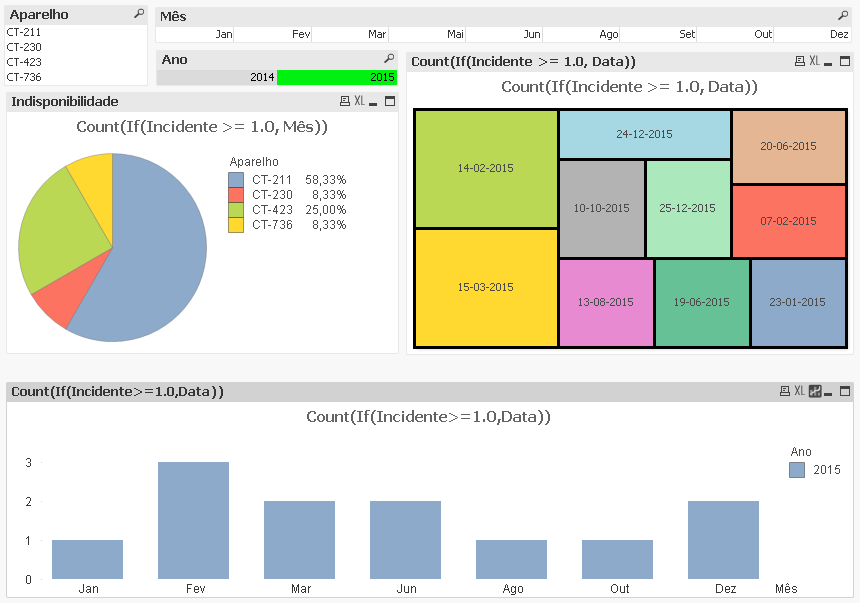
\includegraphics[width=15cm]{qlikview}
\caption{Primeira aplicação em \textit{QlikView}}
\label{fig:qlikViewFig}
\end{figure}
